\section{Introduction}

Atomic chains form one of the prototypical systems in the study of
molecular electronic systems. Atomic nanowires can be fabricated on
inert surfaces~\cite{segovia1999nature,nilius2002science} or in
mechanically controlled break junctions \cite{vanruitenbeek1998mcbj}.
Atomic nanowires are of fundamental scientific interest as they form
electronic one-dimensional systems and for technology they may be viewed
as the limit for metal interconnects in use for nanoelectronics.  Atomic
nanowires are also useful for benchmarking one-dimensional quantum
transport formulations as experiments for these systems provide well
defined and understood conductance values.

Some of the earliest theoretical work with explicit treatment of the
electronic within a quatum transport study of atomic chains is due to
Lang~\cite{Lang1995prb} and this work has served as the prototype for
subsequent studies in molecular tunnel junctions. In this early work,
jellium electrodes are coupled to metal atom chains and the electronic
structure of the system is treated using \ac{DFT}. The Kohn-Sham states
from \ac{DFT} are treated as quasiparticles and the Lippmann-Schwinger
scattering equations are solved for the case of an external voltage bias
applied to the electrodes. Similar scattering approaches in conjunction
with tight binding Hamiltonians applied to the conductance of molecular
junctions combined with Landauer-B\"uttiker theory for electron transport
\cite{emberlykirczenow1999standingwave,
emberlykirczenow2000molecularwire} have been undertaken. 
Subsequently, similar methods have gained prominence by combining a \ac{DFT}
treatment of the electronic structure with a formal \ac{NEGF} treatment of
transport in open systems. More recently, the {\it GW}
approximation~\cite{hedin1965gw} has been introduced to improve  the
quaisparticle description of atomic scale tunnel junctions beyond a Kohn-Sham
description~\cite{RubioThyhgesen,Neaton}.  Use of the
Kohn-Sham energies in the NEGF formulation implies a single determinant
approximation to the many-electron Green's function and similarly the
{\it GW} approximation may be viewed as dynamically screened version of
the Hartree-Fock theory, likewise implying a single determinant
approximation to the many-electron Green's function.  Alternative to
these methods are to use the ideas of exact diagonalization or
configuration interaction in rate equation formulations of electron
transport~\cite{J. N. Pedersen and A. Wacker: Tunneling through
nanosystems: Combining broadening with many-particle states, Physical
Review B 72, 195330 (2005)} or through a many-electron scattering
formulation of the transport problem~\cite{vici2004}. 

In defining models for atomic-scale transport junctions, a partitioning
of the system into semi-infinite electrodes and device region is usually
performed. The device region is given by an explicit model that includes
the device (i.e. atomic chain, molecule, nanowire) as well as a region
that defines the bonding of the device to electrodes, resulting in an
'extended device' or 'extended molecule' region. The portion of the
electrode not explicitly treated by the extended device region is in
most theoretical studies treated by electrode self-energies. In this
approximation, electronic excitations in the electrode region are not
considered. Exceptions to the restriction include
ref.~\cite{galperin2006prl} where the effect of coupling lead
excitations to a two state model of molecular tunnel junction is
explored, or as in a recent formulation of NEGF that allows for
inclusion of electrode interactions to be explicitly
treated~\cite{Ness2011prb}. In the calculations in
ref.~\cite{galperin2006prl}, it is found for certain ranges of electrode
couplings and with left-right asymmetry, that the current arising from
lead excitations can be comparable to the current flowing due to direct
tunneling.

In the following, we apply the method of configuration interaction to a
simple model of electrodes coupled to atomic chain to investigate the
influence of electron correlations on quasiparticle states arising from
the device region, and as well we consider the influence of electrode
excitations as they couple to the device region. This approach enables
us to study the junction in an uncorrelated limit (single determinant
approximation), and to systematically include electron correlations on
the device region and electrodes to study how the quasiparticle states
evolve. By allowing electrode excitations to enter the calculation, we
are able to explore how correlated electrons on the device region
interact with electrode excitations.

%In earlier work~\cite{henderson}, a method was outlined in which an
energy-dependent self-energy is mapped to an energy-independent
\ac{CAP}, which, %when added to the Hamiltonian, can be used in a
many-body treatment of the system. Here, we present a continuation of
that work, applying the method to %a chain of atoms with interacting
electrons, and using a complex \ac{CI} scheme for the calculation of
electronic structure.
%Different levels of correlation are studied by varying the threshold
parameter for \acp{CSF} in the \ac{CI} calculation.

%The rest of this paper is organized as follows: in
section~\ref{sec:method}, we cover the methods used in this work, both
for constructing the \ac{CAP} and %for
%solving the resulting complex symmetric many-body problem. In
section~\ref{sec:results} we present and discuss some results of
applying the
%ormalism to a simple atomic chain system. Finally,
section~\ref{sec:conclusions} contains conclusions and further
perspectives.


\section{Introduction}

Atomic chains form one of the prototypical systems in the study of molecular
electronic systems. They can be fabricated on inert
surfaces~\cite{nilius2002science, segovia1999nature} or in mechanically
controlled break junctions \cite{vanruitenbeek1998mcbj} and are of interest as
potential electronic interconnects, but also because their highly nonclassical
behaviour allows the various theoretical approaches to the one-dimensional
quantum transport problem to be compared with experiment.

Early theoretical approaches to the problem of the conductance of molecular
chains were based on a tight-binding formalism, combined with
Landauer-B\"uttiker theory for transport
\cite{emberlykirczenow1999standingwave, emberlykirczenow2000molecularwire}.
Later on, \ac{DFT}-based methods gained prominence, with conductance
characteristics either inferred from the Friedel sum
rule~\cite{sim2001sodiumwire}, or calculated using the \ac{NEGF}
\cite{meirwingreen1992negf} formalism~\cite{leepuska2004monovalent,
thygesen2003aluminium}. More recently, the GW approximation~\cite{hedin1965gw}
has been introduced as a way of correcting the Kohn-Sham single particle
energies to more closely correspond to the actual quasiparticle energies of the
system~\cite{thygesen_rubio, thygesenrubio2010corr}. Using this formalism,
transport calculations on molecular junctions have been able to achieve
semi-quantitative levels of accuracy~\cite{strange2011benzene,
strange2011alkane}.

However, moethods based on \ac{DFT} + \ac{NEGF} are not the only option for
studying molecular electronic devices. In a different approach, methods from
the field of quantum chemistry, with which it is possible to incorporate
electron correlations to an arbitrary degree can  used \cite{vici2004} but in
those cases, modeling the effect of coupling to leads is problematic. Including
an energy-dependent potential term in the Hamiltonian is possible in principle,
but not feasible in practice.

In earlier work~\cite{henderson}, a method was outlined in which an
energy-dependent self-energy is mapped to an energy-independent
\ac{CAP}, which, when added to the Hamiltonian, can be used
in a many-body treatment of the system. Here, we present a continuation of that
work, applying the method to a chain of atoms with interacting electrons, and
using a complex \ac{CI} scheme for the calculation of electronic structure.
Different levels of correlation are studied by varying the threshold
parameter for \acp{CSF} in the \ac{CI} calculation.

The rest of this paper is organized as follows: in section~\ref{sec:method}, we
cover the methods used in this work, both for constructing the \ac{CAP} and for
solving the resulting complex symmetric many-body problem. In
section~\ref{sec:results} we present and discuss some results of applying the
formalism to a simple atomic chain system. Finally,
section~\ref{sec:conclusions} contains conclusions and further perspectives.


\section{Method}
\label{sec:method}

\subsection{Model System}
\label{subsec:modelsystem}

The system (``device'') we shall study consists of a simple atomic chain with
interatomic separation of 0.28 nm, intended to mirror the system studied
experimentally in~\cite{nilius2002science} (See
figure~\ref{fig:chaincapdevice}). Two interatomic spacings are made larger than
the others, to delineate a ``molecule'' between two leads. This spacing
determines the degree to which the device states couple to the leads, and
variation of the spacing allows us to explore different coupling regimes.

\begin{figure}
	\begin{center}
		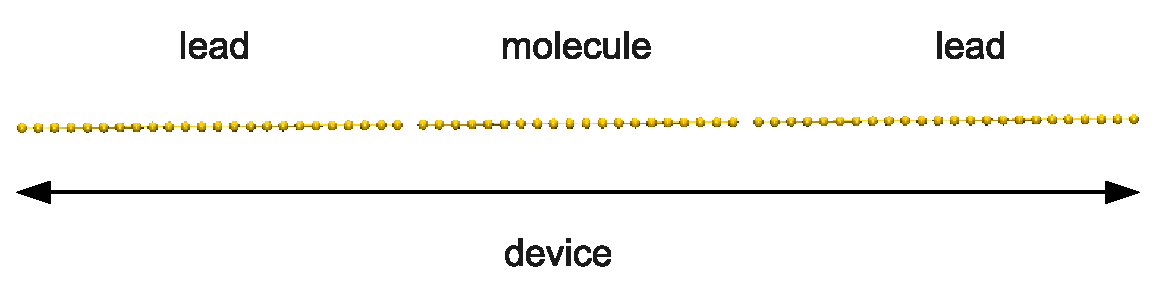
\includegraphics[width=0.9\linewidth]{figures/chaincapdevice}
	\end{center}
	\caption{Model system studied in this work. The molecule consists of 20
	Gold atoms, while the leads consist of 24 atoms each.}
	\label{fig:chaincapdevice}
\end{figure}

For comparison purposes, the transmission spectrum of this system was
calculated in the \ac{NEGF} formalism using the TIMES~\cite{times} code. The
objective is to model the peaks of this spectrum with Lorentzian curves for
which the peak location and peak width are extracted from the real and
imaginary parts, respectively, of the complex eigenvalues obtained by
diagonalization of the Hamiltonian which includes a complex symmetric \ac{CAP}.

\subsection{Complex Absorbing Potential}
\label{subsec:CAP}

The procedure for construction of an energy-independent \ac{CAP} from the
energy-dependant self-energy is discussed in detail in~\cite{henderson}. We
briefly present the essential points here.

The initial Hamiltonian $\um{H}_0$ , with eigenvalues $\varepsilon_i$ and
eigenvectors $\ket{X}_i$, is that of a single unit cell of the semi-infinite
lead. Its self-energy is calculated using the TIMES code~\cite{times}. The
self-energy is adiabatically added to the Hermitian Hamiltonian $\um{H}_0$
leading to the following Dyson equations:

\begin{subequations}
\begin{align}
	[\um{H} + \lambda \um{\Sigma}(\omega_i^\lambda)] \ket{\psi_i^\lambda}
	&= \omega_i^\lambda \um{S}_0 \ket{\psi_i^\lambda} \\
	\bra{\varphi_i^\lambda} [\um{H} + \lambda \um{\Sigma}(\omega_i^\lambda)]
	&= \omega_i^\lambda \um{S}_0 \bra{\varphi_i^\lambda} 
	\label{eq:adiabaticap}
\end{align}
\end{subequations}

% The real part of $\omega_i$ gives the position of the $i$th resonance including
% the shift from the initial eigenvalue $\varepsilon_i$, the imaginary part gives
% the level broadening.
The adiabatic coupling is achieved by varying $\lambda$. At $\lambda = 0$ we
have the initial states $\ket{X}$ and eigenvalues $\varepsilon$, while at
$\lambda = 1$ we have the target states and energy levels.

For the construction of the \ac{CAP}, since our many body code can only deal
with real MO basis sets, we are forced to use the real eigenbasis of \umm{H}
($\um{W}_0$ from \cite{henderson}), defining the \ac{CAP} to be

\begin{equation}
	\um{W} = \um{S}\um{X}\um{\omega}\um{X}^\dagger - \um{H}_0
	\label{eq:capsdef}
\end{equation}

where \umm{\omega} is a diagonal matrix with the complex value $\omega_i$ as
its $i$th diagonal element.

This projection introduces a small amount of inaccuracy, as will be discussed
later. We calculate the transmission through the device region via

\begin{equation}
	T(E) = \mathbf{tr}(\Lambda_L G \Lambda_R G^\dagger)	
	\label{eq:transmission}
\end{equation}

Where generally in the definition of the Green's function, $G$ and spectral
densities, $\Lambda_{L(R)}$ self-energy is used, we replace this with W.

\begin{subequations}
\begin{align}
	G &= [E\um{S}_0 - (\um{H}_0 + \um{W})] \\
	\Lambda_{L(R)} &= i \left( \um{W}_{L,(R)}
	                  - \um{W}^\dagger_{L(R)} \right)
\end{align}
\label{eq:glambdadef}
\end{subequations}

We then analyse the obtained transmission against that using the NEGF formalism
employed within the TIMES code. This comparison is shown in
figure~\ref{fig:transdat}, showing the extent of agreement between the two
approaches. We note the good agreement between the two especially in the energy
frame of interest, \textit{i.e.} around the \ac{HOMO}-\ac{LUMO} gap.

\begin{figure} 
	\begin{center}
		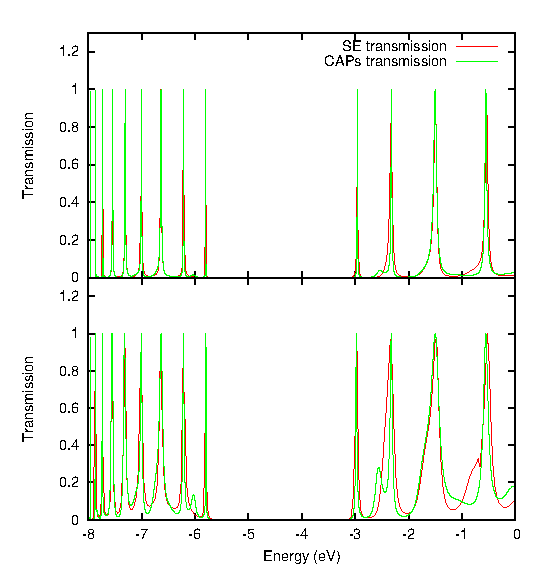
\includegraphics[width=0.9\linewidth]{figures/transdat.eps}
	\end{center}
	\caption{Transmission through the 0.45 nm (top) and 0.40 nm (bottom)
	         systems. The red curve is a transmission spectrum obtained
		 using a conventional self-energy, the green curve is obtained
		 using a \ac{CAP}.}
	\label{fig:transdat}
\end{figure}

% The goal is to introduce a matrix \umm{W} which mimics the effect of coupling
% to a semi-infinite lead in a similar way as a complex self-energy
% \umm{\Sigma(E)}, but without the energy dependence. In order to achieve this,
% we construct \umm{W} such that, when added to the bare Hamiltonian $\um{H}_0$,
% it produces the same set of complex eigenvalues and eigenvectors as the
% Hamiltonian with \umm{\Sigma(E)} added.
% 
% This is achieved by solving the related problem
% 
% \begin{subequations}
% \begin{align}
% 	[\um{H} + \lambda \um{\Sigma}(\omega_i^\lambda)] \ket{\psi_i^\lambda}
% 	&= \omega_i^\lambda \ket{\psi_i^\lambda} \\
% 	\bra{\varphi_i^\lambda} [\um{H} + \lambda \um{\Sigma}(\omega_i^\lambda)]
% 	&= \omega_i^\lambda \bra{\varphi_i^\lambda} 
% 	\label{eq:adiabaticap}
% \end{align}
% \end{subequations}
% 
% for $\lambda$ gradually (adiabatically) increasing from 0 to 1. In this way, we
% go from the eigenenergies and eigenstates of $\um{H}_0$ at $\lambda = 0$ to
% those of $\um{H}_0 + \um{\Sigma(\omega_i)}$ at $\lambda = 1$.


\subsection{Complex Monte Carlo Configuration Interaction}

The \ac{CI} calculations were performed using a version of the \ac{MCCI}
program~\cite{mcci1998, mcci2000} modified according to the orthogonal
projection method outlined in~\cite{tarantelli_csd} to solve the complex
symmetric generalized eigenvalue problem that results when a \ac{CAP} is
introduced into the Hamiltonian. The \ac{MCCI} program computes energy
estimates by an iterative process: starting from a set of \acp{CSF} (which may
be a lone Slater Determinant), a set of \acp{CSF} are created which consist of
single and double excitations from the \acp{CSF} in the current set. These sets
are then joined, and the Schr\"odinger equation is constructed and solved in
the corresponding \ac{CI} subspace. Then follows a pruning step, in which those
\acp{CSF} which have a coefficient in the relevant eigenvector of the
Hamiltonian lower (in magnitude) than a given threshold value $cmin$ are
deleted, after which the process is repeated until convergence is reached.

To explore the effect of electron correlation on the shifts and broadenings,
lower values of the threshold parameter $cmin$ can be chosen, admitting more
\acp{CSF} to the final solution.
% Only those \acp{CSF} which excited into or from states localized in the device
% (as opposed to the part of the leads which is included in the device region)
% were considered, since we wanted to explore only excitations of the actual
% device.

\subsection{Complex Quasiparticle Energies}

We evaluate quasiparticle energies as differences of complex many-body energies
that result from the \ac{CI} problem, as discussed above. In order to compare
to transmission spectra from the single-particle picture, we construct
Lorentzian peaks from the complex energies $\omega_i$ according to

\begin{equation}
	f(\varepsilon;\omega_i)
	= \frac{\left( \frac{\Gamma}{2} \right)^2}
	       {(\varepsilon - \operatorname{Re}(\omega_i))^2
	       + \left( \frac{\Gamma}{2} \right)^2}
	\label{eq:lobro}
\end{equation}

where $\Gamma = 2 \times \operatorname{Im}(\omega_i)$ is the broadening
associated with the eigenvalue (i.e. the width of the Lorentzian peak).

\section{Results and Discussion}
\label{sec:results}

\subsection{Single-Particle Picture}
\label{subsec:SingleParticle}

As a validation of the \ac{CAP} approach, we would first like to see whether
the \ac{CAP} as generated according to the description of
section~\ref{subsec:CAP} gives the correct complex single-particle eigenvalues,
i.e. whether the selected self-consistent solutions of the Dyson
equations~\ref{eq:adiabaticap} provide an accurate picture of the resonances
in the device region. To do this, we construct Lorentzian peaks from the
eigenvalues, and compare to a transmission spectrum of the device obtained
using the self-energy in the \ac{NEGF} formalism. Such a comparison is shown in
figure~\ref{fig:13evals}.

This is a case of weak coupling, as can be seen by the narrowness of the
transmission peaks, and by the fact that they are not significantly shifted
from the real-valued Hartree-Fock single-particle levels. The agreement between
the Green function transmission (red) and the peaks derived from the
eigenvalues of $\um{H}_0 + \um{W}$ (green) is excellent, both in terms of
position (real part) and width (imaginary part). In the inset, the region
around the \ac{HOMO} is plotted in detail, showing the extent of the agreement
between the two methods (the green and red curves practically overlap).

\begin{figure} 
	\begin{center}
		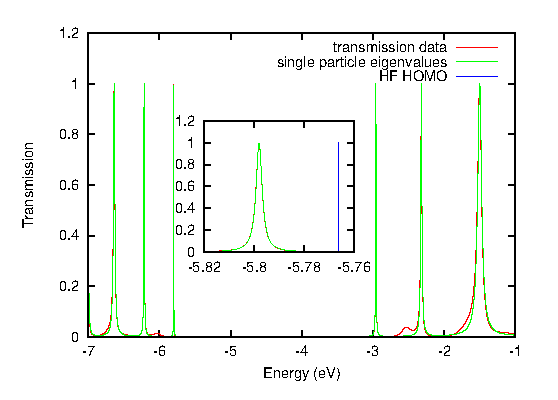
\includegraphics[width=0.9\linewidth]{figures/13evals}
	\end{center}
	\caption{Comparison of transmission data (red) with Lorentzian
	broadened complex eigenvalues of $\um{H}_0 + \um{W}$ (green) for a
	model system as described in section~\ref{subsec:modelsystem}, with
	device-lead gap of 0.45 nm. Transmission data was obtained from
	\ac{NEGF} calculations with the TIMES program~\cite{times}.
	The inset shows a close-up view of the \ac{HOMO}, with the HF \ac{HOMO}
	shown in blue for reference.
	}
	\label{fig:13evals}
\end{figure}

\subsection{Single Determinant}
\label{subsec:SingleDeterminant}

The next step is to pass to the many-body picture, initially representing the
many-body wave function of the system as a single Slater determinant. The
quasiparticle peaks in the transmission spectrum are approximated by taking
differences of many-body energies: $E^N - E^{N-1}$ yields the \ac{HOMO}, while
likewise $E^{N+1} - E^N$ yields the \ac{LUMO} (other quasiparticle levels can be
obtained by taking differences of excited many-body energies). The peaks for
the \ac{HOMO} and \ac{LUMO} of the system obtained in this way are plotted in
figures~\ref{fig:nobranch45A} and \ref{fig:nobranch40A}. There is good
correspondence in the position of the peaks, but the single determinant
difference peaks are significantly broader than their transmission spectrum
counterparts. The only difference with the single-particle eigenvalue picture
previously shown is that now, as mentioned earlier, we have projected the
eigenvectors into the $\um{X}$ basis (eigenbasis of $\um{H}_0$) instead of
representing them in their natural basis $\um{U}$ (left eigenbasis of
$\um{H}_0 + \um{W}$).
% The reason for this is that our \ac{CI} code is constrained to work with a real
% basis of MOs.

\begin{figure}[h]
	\begin{center}
		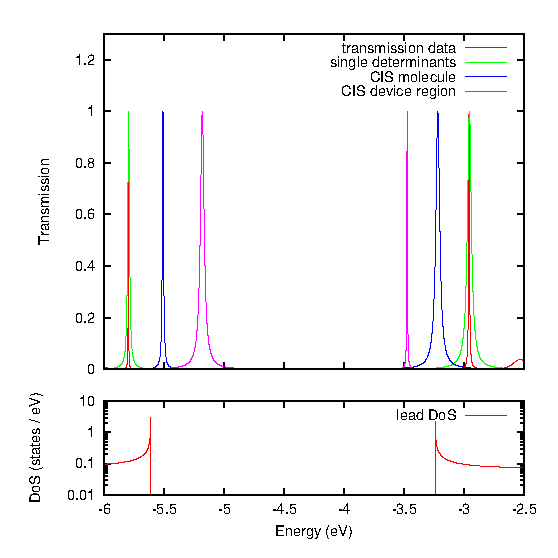
\includegraphics[width=0.9\linewidth]{figures/nobrsingles45A.eps}
	\end{center}
	\caption{4.5A system: Comparison of the transmission from Green
                 functions (red) to the Lorentzian peaks obtained by
                 subtracting single-determinant many-body energies (green).}
	\label{fig:nobranch45A}
\end{figure}

\begin{figure}[h]
	\begin{center}
		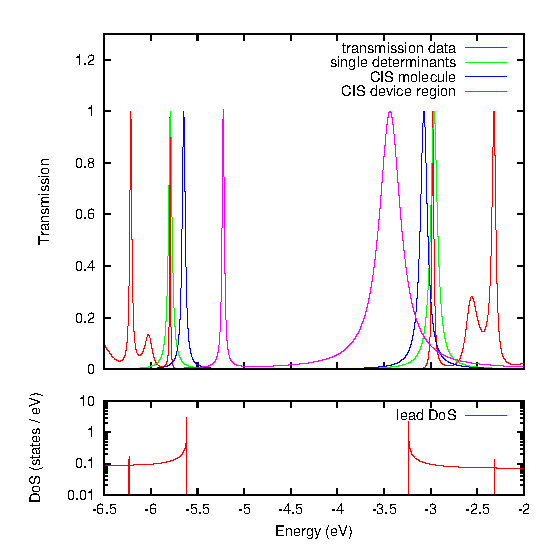
\includegraphics[width=0.9\linewidth]{figures/nobrsingles40A.eps}
	\end{center}
	\caption{4.0A system: Comparison of the transmission from Green
                 functions (red) to the Lorentzian peaks obtained by
                 subtracting single-determinant many-body energies (green).}
	\label{fig:nobranch40A}
\end{figure}

\subsection{Single Excitations}
\label{subsec:singles}

The next step is to include, for each state, the reference determinant plus all
its single excitations. By Thouless' theorem~\cite{Thouless}, to first order in
the coefficients of the non-reference \acp{CSF}, the wave function obtained by
diagonalizing in this space would still be describable as a single determinant
(and thus, by definition, contain no correlation), but by adding degrees of
freedom to the system, a degree of self-consistency is attained. This is similar
to a $\Delta$-SCF calculation, where many-body energies of different particle
number are compared at the SCF level.

We make a distinction between two types of ``singles'' \ac{CI} vectors: for the
``molecule'' calculations, the \ac{CI} space was truncated to contain only
excitations from and to MOs of the molecule (this set was found by comparing
the real parts of the complex eigenvalues $\omega_i$ with the positions of the
peaks of the respective transmission spectrum). The ``device region''
calculations contain the full singles \ac{CI} vector, i.e. all single
excitations plus the reference determinant. The results are plotted in
figures~\ref{fig:nobranch45A} and \ref{fig:nobranch40A}.

At this point, it is useful to compare the error in the two cases discussed
thus far. To relate the many-body energies to the single-particle levels, we
start by considering the following equation for the total energy of the system
(which we assume to be closed-shell) in terms of complex single-particle
energies

\begin{equation}
	E = \sum_i \omega_i - \frac{1}{2} \sum_{i,j} g_{ij}
	\label{eq:sptotalenergy}
\end{equation}

which reflects the fact that when summing the single particle energies, the
two-body terms are counted twice and must be subtracted out to obtain the total
energy. On the other hand, from the many-body point of view, we have

\begin{equation}
	E_{mb} = \sum_i h_i + \frac{1}{2} \sum_{i,j} g_{ij}.
	\label{eq:mbtotalenergy}
\end{equation}

It follows that

\begin{equation}
	\sum_i \omega_i = E_{mb} + \frac{1}{2} \sum_{i,j} g_{ij}.
	\label{eq:eesumcomparison}
\end{equation}

In other words, we can compare the obtained many body energies in both the
single determinant and single excitations cases, and determine whether the
additional degrees of freedom are able to compensate the error inherent in the
basis conversion. Such comparisons are meaningful since the single excitations
vector contains no correlation energy, but that would not be the case in a more
extensive \ac{CI} scheme. Table \ref{tab:eesum} contains the comparisons for
the 0.45 nm system with 68 electrons.

% FULL PRECISION VALUES
%               & single determinant & single excitations & $\sum \omega_i$ \\
%   real part      & -17.978662182501026 & -17.979628470130947 & -17.978417894\\
%   imaginary part & -0.12546017404575291 & -0.1252335053564404 & -0.1252903752532\\
\begin{table}
  \centering
  \begin{tabular}{l r r r} 
    \hline
                 & single determinant & single excitations & $\sum \omega_i$ \\
    \hline
    real part      & -17.97866 & -17.97962 & -17.97841\\
    imaginary part & -0.12546 & -0.12523 & -0.12529\\
    \hline
  \end{tabular}
  \caption{Comparison of many-body energies (columns 1 and 2) with
           single-particle levels (column 3).}
  \label{tab:eesum}
\end{table}

For the single determinant case, we obtain good agreement in the real part, but
a significant error in the imaginary part, consistent with behaviour plotted in
figure~\ref{fig:nobranch45A}. Again, this is due to the real basis not being 
well able to reproduce imaginary eigenvectors. For the single excitations case,
the situation is reversed; for the real part we get an error which we ascribe
to the finite expansion (Thouless' theorem is strictly only valid in an
infinite basis), whereas for the imaginary part we get good agreement, due to
the fact that our complex \ac{CI} code was able to assign complex coefficients
to the \acp{CSF} and thus reproduce the imaginary part of the energy better.

\subsection{Complex \ac{CI}}

We now move on to the \ac{CI} results, where the criterion for inclusion of a
\ac{CSF} in the \ac{CI} vector is simply its coefficient in the wave function,
and the threshold is a program parameter which can be varied to include a given
amount of correlation. The results for both systems have been plotted together,
in figure~\ref{fig:cihomo} for the \ac{HOMO}, and figure~\ref{fig:cilumo}
for the \ac{LUMO}. The curves labeled ``unrestricted'' indicate that the \ac{CI}
procedure was not limited to MOs on the molecule; MOs localized on the lead
sections of the device were also included. Note that in this case, the QP gap
widens as compared to the HF case, which would seem to be in contrast to
earlier findings which indicated that screening effects on the metal leads
renormalize the levels of the device, leading to lower
gaps~\cite{thygesen_rubio, thygesen}. This behaviour persists however, in
\ac{CI} calculations performed on the system in absence of a \acp{CAP},
indicating that this is a physical effect.

As can be seen in the figures, the \ac{CI} gap is slightly smaller than the HF
gap, and decreases with increasing correlation, consistent with the HF and GW
results in~\cite{thygesen_rubio, thygesenrubio2010corr}. In both cases the peak
widths are larger than the corresponding transmssion (HF) peaks, but similar
to the single excitations peaks, indicating that the broadening is accurately
captured at the level of single excitations.

\begin{figure}
	\begin{center}
		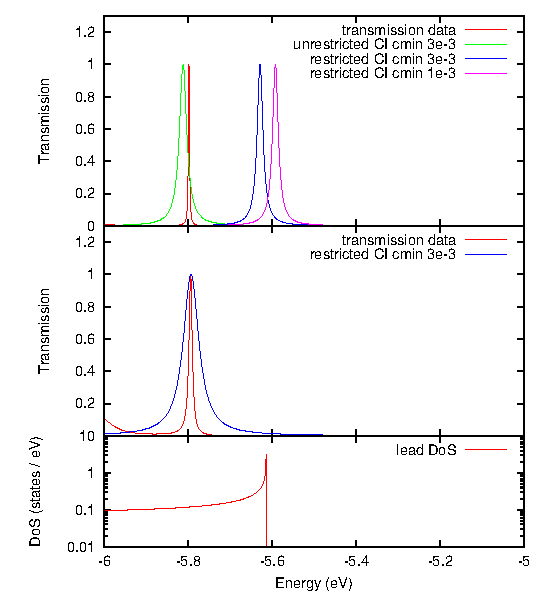
\includegraphics[width=0.9\linewidth]{figures/cihomo.eps}
	\end{center}
	\caption{CI for the \ac{HOMO} of the 0.45 (top) and 0.40 nm (middle)
                 systems, with the Density of States of the leads plotted
                 below.}
	\label{fig:cihomo}
\end{figure}


\begin{figure}
	\begin{center}
		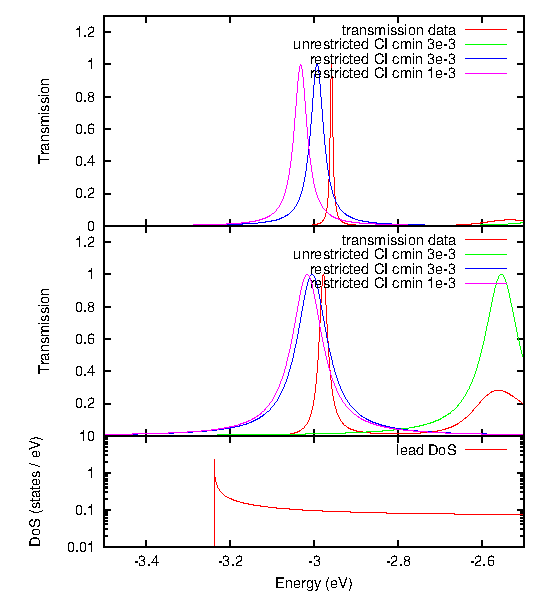
\includegraphics[width=0.9\linewidth]{figures/cilumo.eps}
	\end{center}
	\caption{CI for the \ac{LUMO} of the 0.45 (top) and 0.40 nm (middle)
                 systems, with the Density of States of the leads plotted
                 below.}
	\label{fig:cilumo}
\end{figure}

\section{Conclusions}
\label{sec:conclusions}

In this work we presented what to our knowledge are the first application
of wavefunction methods to the study of semi-infinite systems using acomplex
absorbing potential. For different degrees of molecule-lead coupling and
different levels of correlation, the complex quasiparticle peaks of a system
consisting of atomic gold chains were evaluated.

The ability to accurately describe these levels (which in this case
correspond to \ac{IP} and \ac{EA}) has been shown to be closely related to an
accurate description of transport~\cite{golden}. This work opens the door for
the application of non-empirical wave funcion methods to the study of quantum
transport in nanoscale systems in which the lifetime broadening is captured
accurately by a self-energy-derived \ac{CAP}.
